\documentclass{article}

\usepackage[affil-it]{authblk} 
\usepackage{geometry}
\usepackage{hyperref}
\usepackage{graphicx}
\usepackage{amsmath}
 \geometry{
 a4paper,
 total={160mm,257mm},
 left=20mm,
 top=20mm,
 }

\begin{document}
\title{\large DSGA 1013 Final Project Proposal}
\author{\small Alec Hon, Andrew Yeh}
\date{\footnotesize \today}
\maketitle

\section{Introduction}

Wavelets, or 'small waves', are a family of zero mean functions that are used mostly in signal processing, with all wavelets being characterized by starting with zero amplitude, followed by an increase in amplitude, and then a final decrease in amplitude back to zero over a small time scale. 
\begin{figure}[h]
\caption{Haar Mother Wavelet with Example Translations and Dilations}
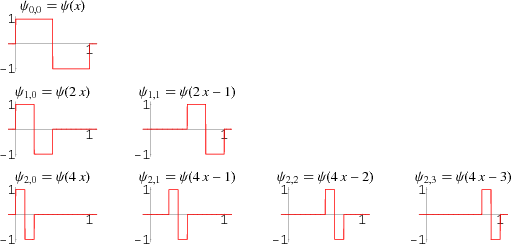
\includegraphics[scale = 0.6]{img/haar_2.png}
\centering
\end{figure}

\noindent
While Fourier Transforms are powerful in representing a function across the entire time domain by transforming a function into trigonometric polynomials, they struggle with studying functions over a local time space as many extra coefficients need to be added into the Fourier Transform of a function to effectively cancel out all the amplitude outside the area of study (\href{https://www.ams.org/journals/bull/1993-28-02/S0273-0979-1993-00390-2/S0273-0979-1993-00390-2.pdf}{Strang, 1993}). On the other hand, wavelet analysis expands a function into translations and dilations of a mother wavelet function and allow the study of functions at a local time range,  making it possible to recreate functions that include abrupt changes with fewer coefficients at a local space than a Fourier transform. Wavelets have been used in image processing, with a large amount of study being focused on image compression and denoising.  
 \newline
 
\noindent In this project, we wish to study the use of wavelet decomposition as a pooling technique in Convolutional Neural Networks (CNNs) as a method for improving image classification in CNNs. Conventional CNN pooling techniques include max pooling and mean pooling, with both pooling techniques showing shortcomings, as details in images are either diluted or lost upon using either pooling algorithm. Other pooling methods include mixed pooling, where max pooling or mean pooling is randomly selected at every convolved field as investigated in \href{https://openreview.net/pdf?id=rkhlb8lCZ}{Williams, Li (2018)}. Since wavelets are particularly useful in studying signals at a local level, we can consider the convolved field as a local region in an image in which we can use wavelets to decompose each field and return its approximation or detail coefficient as a pooling technique. We define the two-dimensional discrete wavelet transform as:
\begin{align*}
W_{\text{approximation}}(a,p,q) &= \frac{1}{\sqrt{PQ}}\sum_{x=0}^{P-1}\sum_{y=0}^{Q-1}f(x,y)\varphi_{a,p,q}(x,y)\\
W_{\text{detail}}(a,p,q) &= \frac{1}{\sqrt{PQ}}\sum_{x=0}^{P-1}\sum_{y=0}^{Q-1}f(x,y)\Psi_{a,p,q}(x,y)
\end{align*}
where $f(x,y)$ is an image with dimensions $P\times Q$, resolution level $a$, subband dimensions $p$ and $q$. The approximation transform is what we are primarily interested in capturing.
\newline
\newline

\noindent
We hypothesize that this will capture more information than either max or mean pooling techniques, and lead to more accurate image classifiers. In fact, it has been shown that wavelet decomposition as a pooling technique on convolved layers is an effective technique in image classification, particularly with the Haar Wavelet and the Symlet Wavelet, as shown by \href{https://link.springer.com/chapter/10.1007/978-3-319-76351-4_31}{Chaabane, Mellouli, Hamdani, et.\ al (2018)} and \href{https://arxiv.org/pdf/1805.08620.pdf}{Fujieda, Takayama, Hachisuka (2018)}. As a result, we want to study the usage of different mother wavelets for decomposition as a pooling technique in image classification first for greyscaled images, and then for color images. Our methodology is described below:

\section{Methodology}
\begin{enumerate}
\item Our first goal is to closely recreate the results of \href{https://link.springer.com/chapter/10.1007/978-3-319-76351-4_31}{Chaabane, Mellouli, Hamdani, et.\ al (2018)} in constructing a CNN with wavelet decomposition as a pooling method, utilizing the MNIST dataset as a method to test effective accuracy of wavelet decomposition in image classification. By doing this, we will show that we are able to utilize wavelet decomposition effectively in a CNN. We will compare our accuracies of the wavelet decomposition pooling technique with the standard max, mean, and mixed pooling techniques to see whether or not the wavelet decomposition pooling creates CNNs with higher accuracy. 
\item We then explore the usage of different wavelet families utilizing the PyWavelet Package for the decomposition step in pooling, seeing which wavelet family allows the CNN to classify more accurately. For example, \href{https://easychair.org/publications/download/6Mbb}{Rosetto and Zhou (2019)} investigate using the Shannon wavelet. Afterwards, time permitting, we will attempt to perform the wavelet decomposition for color images, utilizing the CIFAR-10 dataset for classification. By applying different wavelets on different training sets and seeing the difference in classification results, we hope to understand the effects of wavelet pooling on CNNs and the robustness of the results.
\end{enumerate}



\end{document}
